\documentclass[12pt]{article}

\usepackage[13643]{easymcm}  % Team control number
\usepackage{longtable}
\usepackage{booktabs}

\problem{A}  % Problem number

\title{Paper Name}  % Title

\begin{document}

\begin{abstract}

	Some random text
	
\end{abstract}

\maketitle
\tableofcontents

\section{Introduction}

	\subsection{Problem Background}
	
	\subsection{Problem Restatement}
	
	some random text

\section{Dandelion Spread Model}

	\subsection{Assumptions and Justifications}
	
	good
	
	\subsection{Environmental Factors}
	
	\subsection{Dandelion Life Cycle}
	
	\subsection{Dispersal Distance}
	
	\subsection{Algorithm}
	
	\subsection{Dandelion Spread Results}
	
		\subsubsection{Results}
		
		text
		
		\begin{figure}
			\centering
			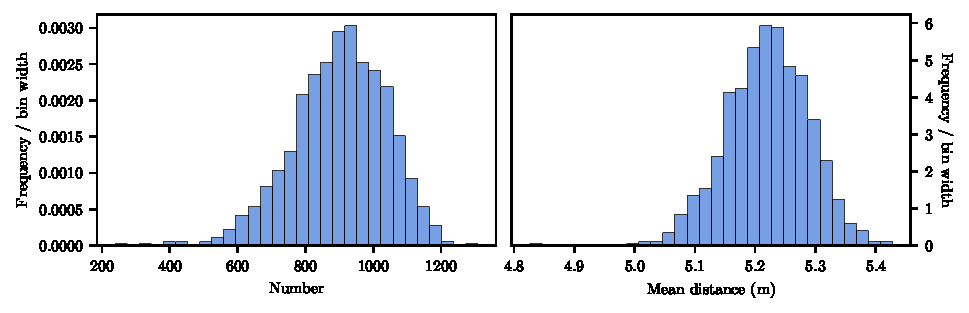
\includegraphics{number-frequency.pdf}
			\caption{Frequency distribution of number and mean distance of dandelions in Florida}
			\label{fig:freq}
		\end{figure}
		
		
		\begin{figure}
			\centering
			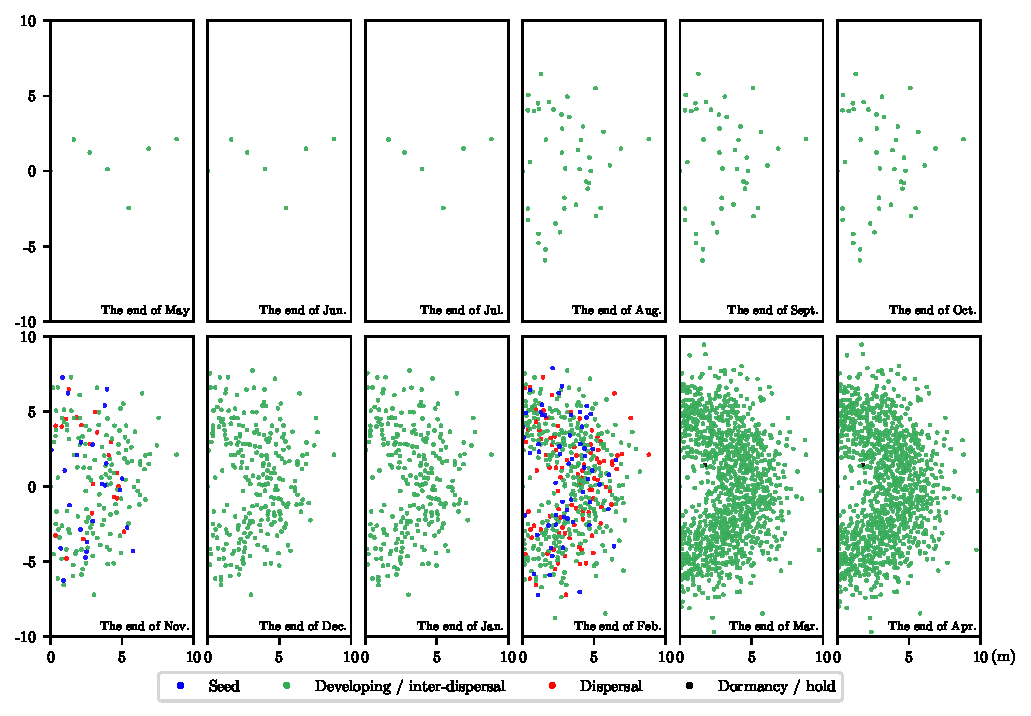
\includegraphics{spread_course-time.pdf}
			\caption{The spread of dandelion during a 12-month period in Florida}
			\label{fig:spread}
		\end{figure}
		
		Lorem ipsum dolor sit amet Lorem ipsum dolor sit amet Lorem ipsum dolor sit amet Lorem ipsum dolor sit amet Lorem ipsum dolor sit amet Lorem ipsum dolor sit amet Lorem ipsum dolor sit amet Lorem ipsum dolor sit amet Lorem ipsum dolor sit amet Lorem ipsum dolor sit amet Lorem ipsum dolor sit amet Lorem ipsum dolor sit amet Lorem ipsum dolor sit amet Lorem ipsum dolor sit amet Lorem ipsum dolor sit amet Lorem ipsum dolor sit amet Lorem ipsum dolor sit amet Lorem ipsum dolor sit amet Lorem ipsum dolor sit amet Lorem ipsum dolor sit amet Lorem ipsum dolor sit amet Lorem ipsum dolor sit amet Lorem ipsum dolor sit amet Lorem ipsum dolor sit amet Lorem ipsum dolor sit amet Lorem ipsum dolor sit amet Lorem ipsum dolor sit amet Lorem ipsum dolor sit amet Lorem ipsum dolor sit amet Lorem ipsum dolor sit amet Lorem ipsum dolor sit amet Lorem ipsum dolor sit amet Lorem ipsum dolor sit amet Lorem ipsum dolor sit amet Lorem ipsum dolor sit amet Lorem ipsum dolor sit amet Lorem ipsum dolor sit amet Lorem ipsum dolor sit amet Lorem ipsum dolor sit amet Lorem ipsum dolor sit amet Lorem ipsum dolor sit amet Lorem ipsum dolor sit amet Lorem ipsum dolor sit amet Lorem ipsum dolor sit amet Lorem ipsum dolor sit amet Lorem ipsum dolor sit amet Lorem ipsum dolor sit amet Lorem ipsum dolor sit amet Lorem ipsum dolor sit amet Lorem ipsum dolor sit amet Lorem ipsum dolor sit amet Lorem ipsum dolor sit amet Lorem ipsum dolor sit amet Lorem ipsum dolor sit amet Lorem ipsum dolor sit amet Lorem ipsum dolor sit amet Lorem ipsum dolor sit amet Lorem ipsum dolor sit amet Lorem ipsum dolor sit amet Lorem ipsum dolor sit amet 
		
		\subsubsection{Sensitivity Analysis}
		
		\subsubsection{Strengths and Weaknesses}
		
	\subsection{Dandelion Spread Fitting Model}
		
		\subsubsection{Data}
		
		\subsubsection{Algorithm}
		
		\subsubsection{Results}
		
		\subsubsection{Sensitivity Analysis}
		
		\subsubsection{Strengths and Weaknesses}
	
		some random text
		
\section{Plant Impact Factor Model}

	\subsection{Assumptions and Justifications}
	
	\subsection{Model Description}

	hello
	
	{
	\fontsize{10}{13}\selectfont
	{
	\begin{longtable}{p{0.5in}p{1.7in}p{3.8in}}
	
	\toprule
	\multicolumn{1}{c}{\textbf{Symbol}} 
		& \multicolumn{1}{c}{\textbf{Aspect}}
		& \multicolumn{1}{c}{\textbf{$a_i$, $b_i$ and $c_i$ Evaluation}} \\

	\toprule
	\multicolumn{3}{l}{Plant Characteristics}\\
	\midrule
	
	$A_1$ & Duration & $a_1=0.5$ (Annual), $0.75$ (Biennial), $1$ (Perennial)\\
	$A_2$ & Growing Habit & $a_2=0$ (Tree), $0.25$ (Shrub), $0.5$ (Vine), $0.75$ (Graminoid), $1$ (Forb/herb)\\ 
	$A_3$ & Growth Rate & The growth rate after successful establishment\\
		& & $a_3=0.5$ (Slow), $0.75$ (Moderate), $1$ (Rapid)\\
	$A_4$ & Lifespan & $a_4=0.25$ (when $a_1=0.5$ or $0.75$), $0.5$ (Short), $0.75$ (Moderate), $1$ (Long) \\
	$A_5$ & Fertility Requirement & Relative level of nutrition (N, P, K) required for normal growth and development.\\
		 & & $a_5=0.5$ (Low), $0.75$ (Medium), $1$ (High)\\
	$A_6$ & Fruit/Seed Abundance & The amount of seed produced.\\
		& & $a_6=0.25$ (None), $0.75$ (Low), $0.75$ (Medium), $1$ (High)\\
	$A_7$ & Propagated Methods & The propagetion methods  \\
	$A_8$ & Seed Spread Rate & hello \\
	$A_9$ & Seedling Vigor & hello \\
	
	\midrule
	\multicolumn{3}{l}{Human and Environment}  \\
	\midrule
	
	$B_1$ & Toxicity & hello \\
	$B_2$ & Product & hello \\
	$B_3$ & Palatable Animal & hello \\
	$B_4$ & Palatable Human & hello \\
	$B_5$ & Commercial Availability & hello \\

	\midrule
	\multicolumn{3}{l}{Location}  \\
	\midrule
	
	$C_1$ & Soil Adaption & hello \\
	$C_2$ & Temperature Adaption & hello \\
	$C_3$ & Humid Adaption & hello \\
	$C_4$ & Population Density  & hello \\

	\bottomrule
	
	\end{longtable}
	}
	}

	hello!!! \\

	\subsection{Sensitive Analysis}

	\subsection{Strengths and Weaknesses}

	some random text
	
\section*{We Share the Earth}
\addcontentsline{toc}{section}{We Share the Earth}



\newrefcontext
\printbibliography

\end{document}
